\begin{frame}
  \frametitle{V\&V Study 2: MSRE Pump Start-up \& Coast-Down Transients}
  Numerical study based on two transient flow-rate tests on the MSRE under zero-power
  conditions. Starting from zero-power critical states with/without forced flow, the fuel salt pump
  was coasted down/started up.
  \begin{columns}
    \column[t]{5.5cm}
    \begin{figure}
      \centering
      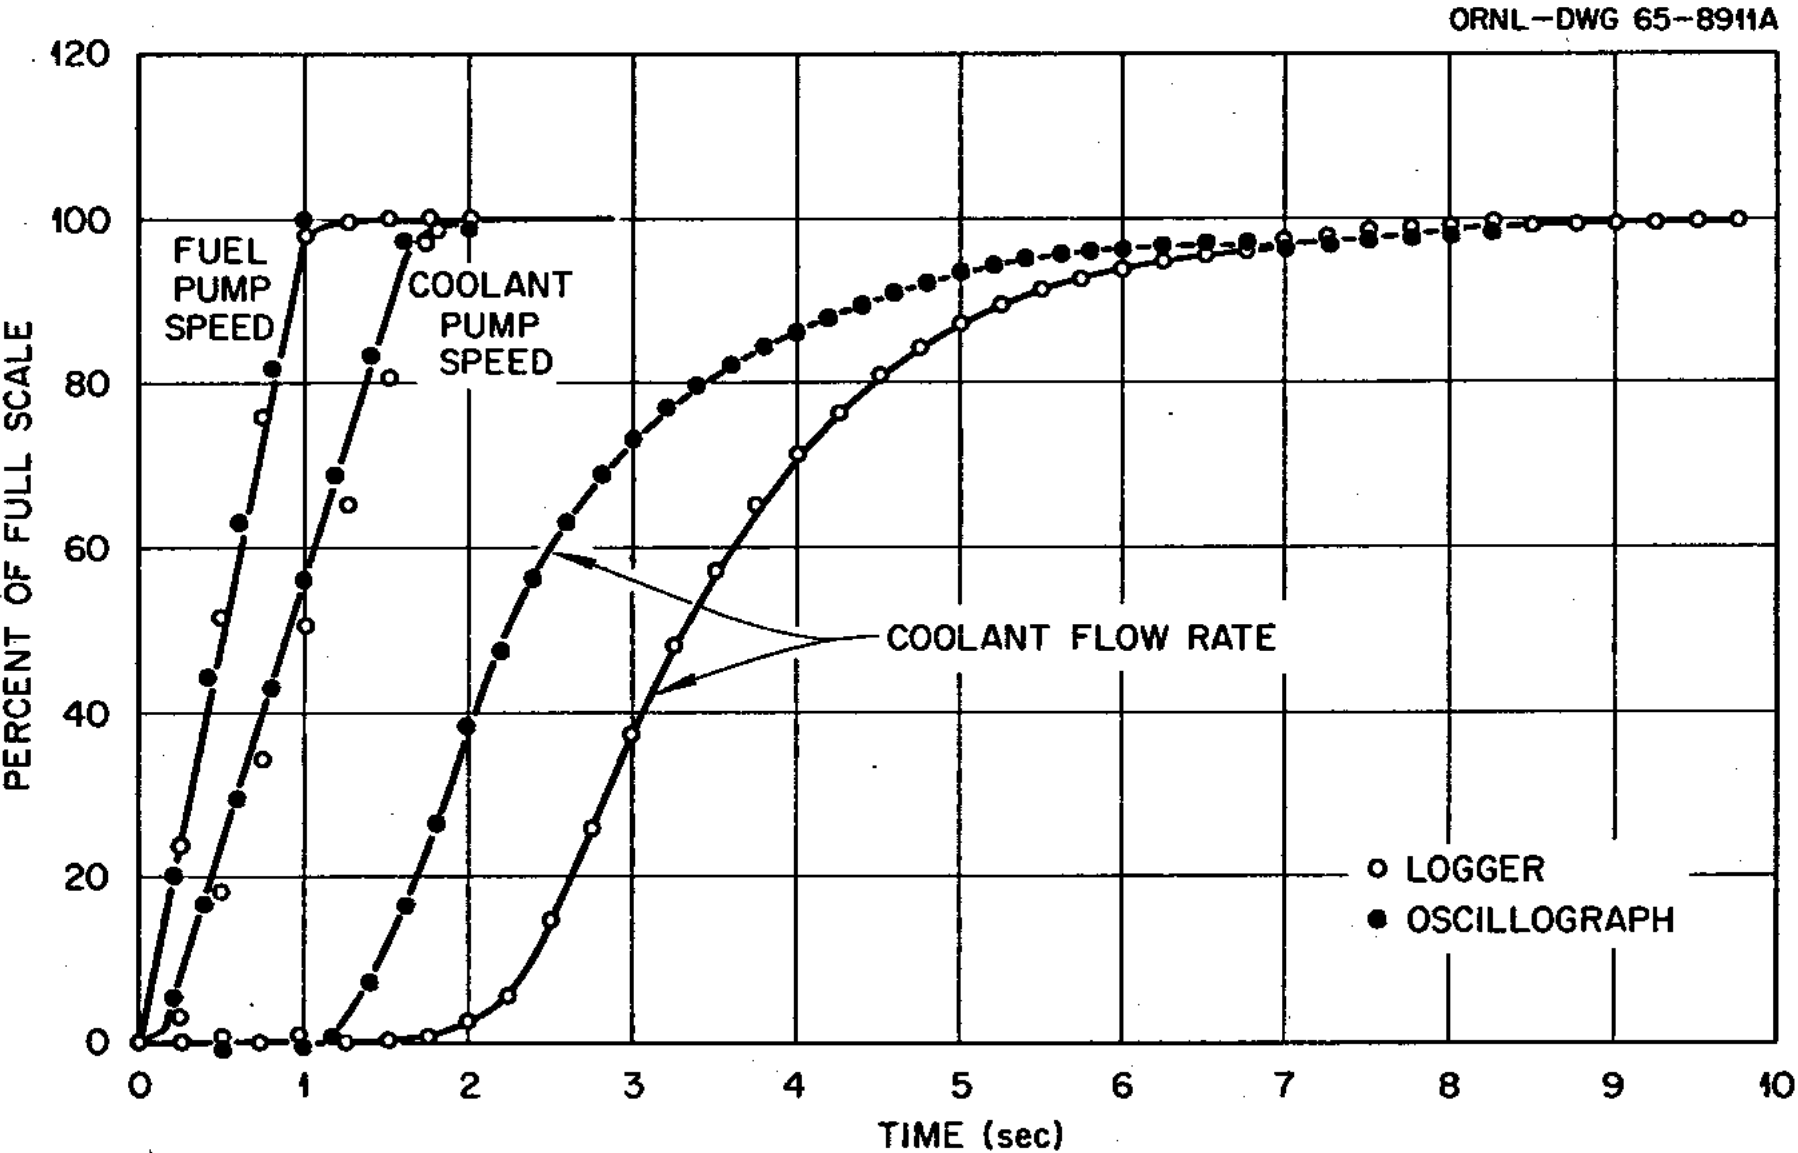
\includegraphics[width=.8\columnwidth]{images/msre-startup}
      \caption{MSRE start-up pump speed and flow rate experimental data
      \cite{prince_zero-power_1968}.}
    \end{figure}
    \column[t]{5.5cm}
    \begin{figure}
      \centering
      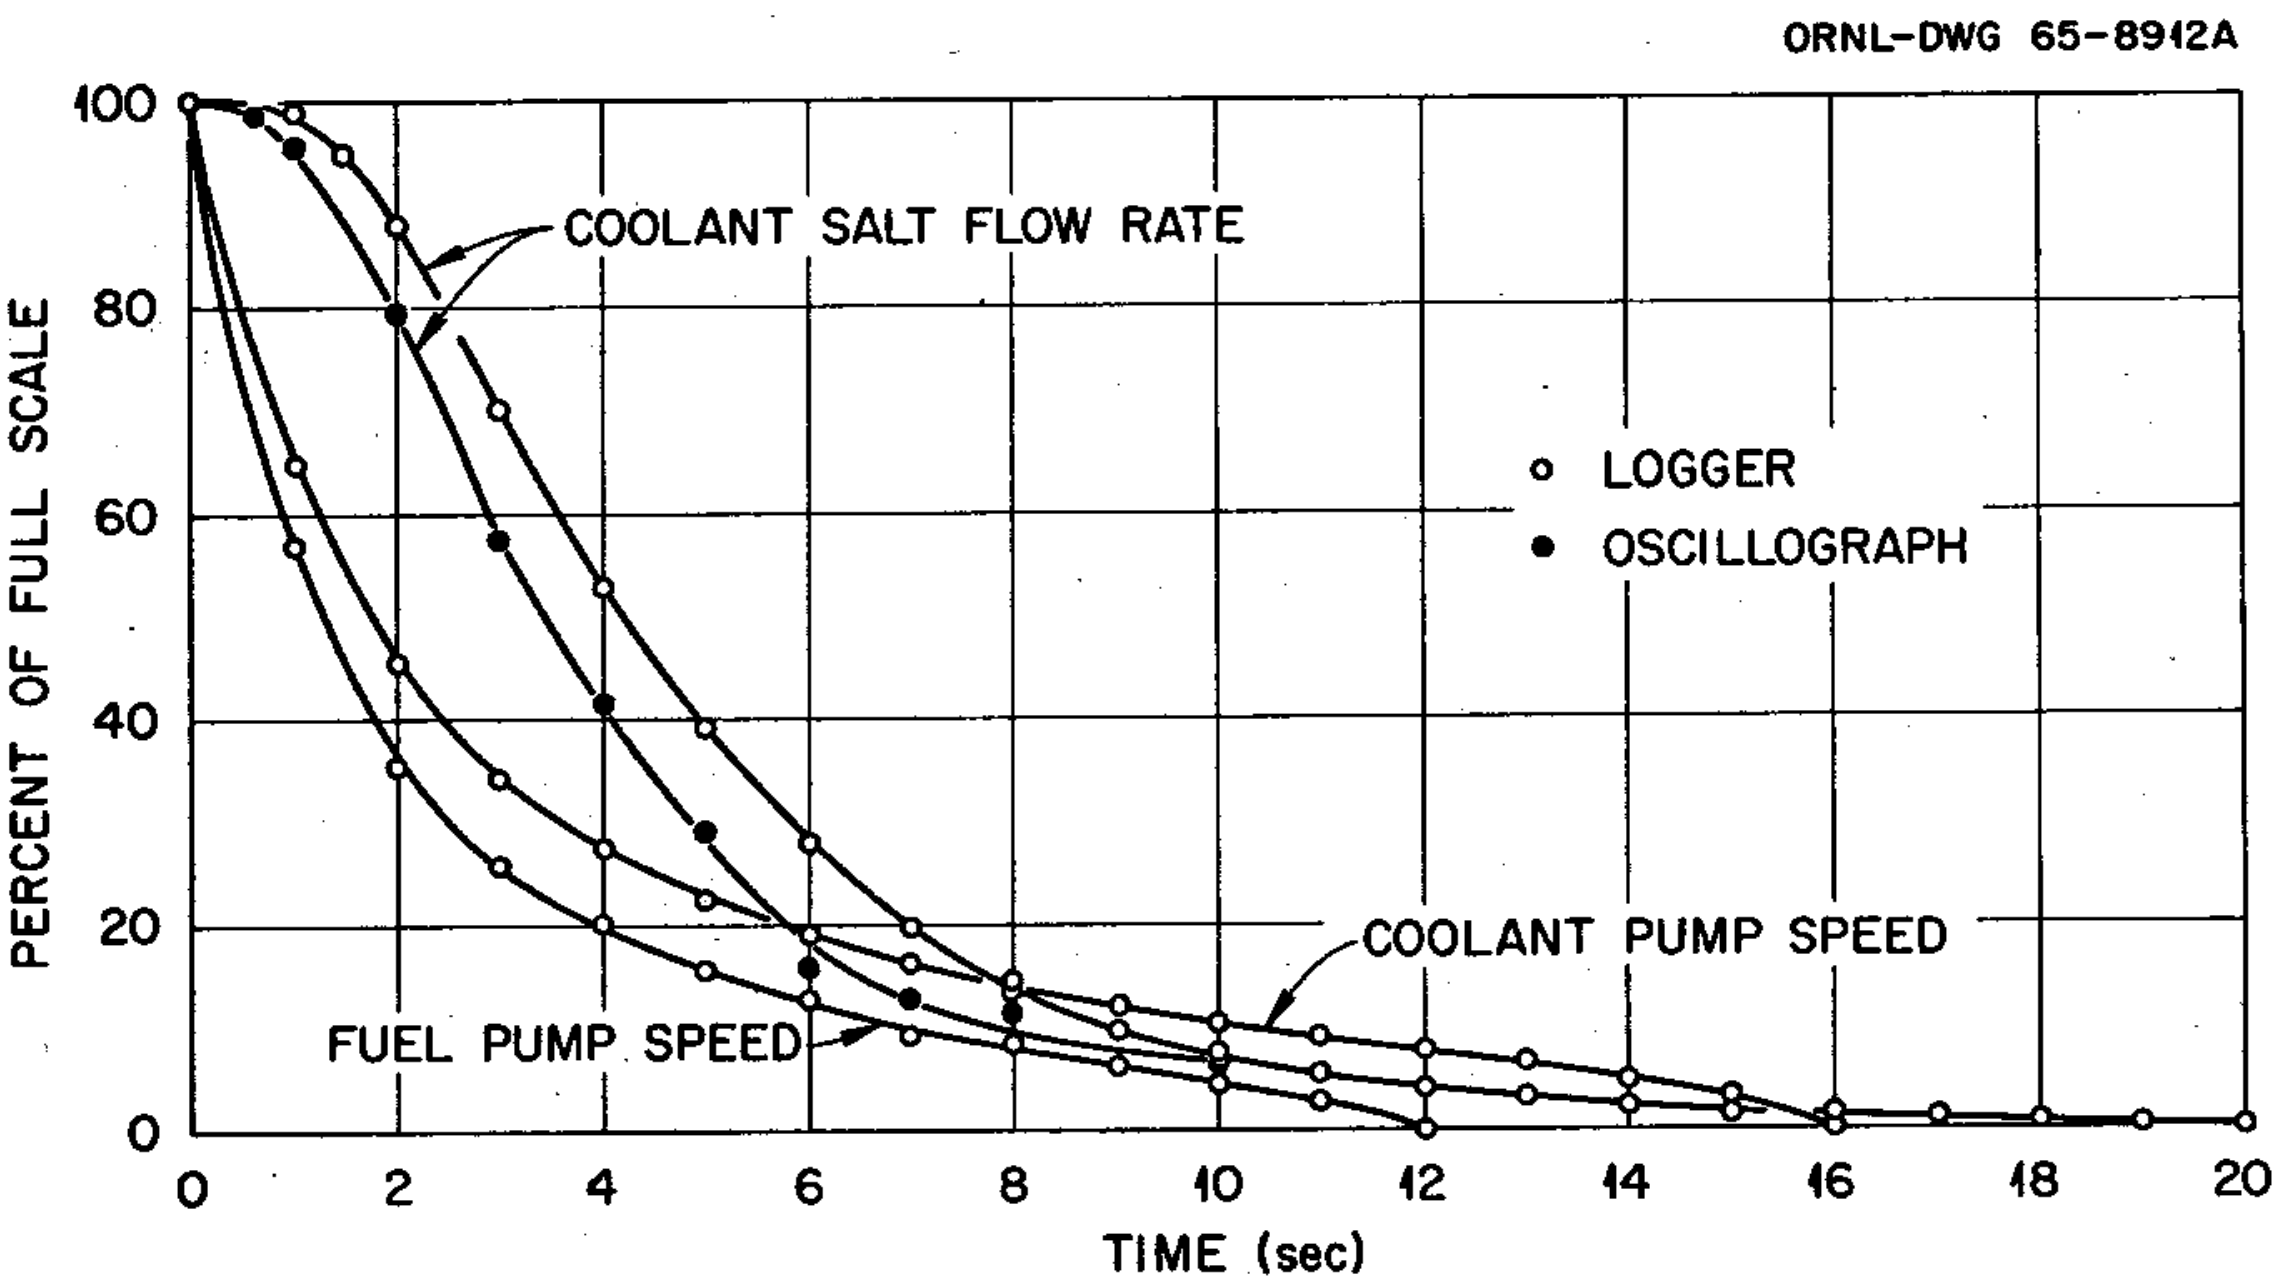
\includegraphics[width=.95\columnwidth]{images/msre-coastdown}
      \caption{MSRE coast-down pump speed and flow rate experimental data
      \cite{prince_zero-power_1968}.}
    \end{figure}
  \end{columns}
\end{frame}

\begin{frame}
  \frametitle{V\&V Study 2: MSRE Pump Start-up \& Coast-Down Transients}
  \begin{block}{\textbf{MSR Phenomena Involved}}
    \begin{itemize}
      \item DNP drift under time-varying flow
      \item Loss of delayed neutrons due to out-of-core DNP decay
    \end{itemize}
  \end{block}
  \begin{block}{\textbf{Aim of the Study}}
    Reproduce the reactivity curve of the control rod response with a 2-D axisymmetric model of the
    MSRE in Moltres.
  \end{block}
  \begin{block}{\textbf{Study Objectives}}
    \begin{itemize}
      \item Develop a verification benchmark based on the MSRE pump start-up \& coast-down
        transients that is easily reproducible
      \item Verify Moltres against QuasiMolto in collaboration with Aaron Reynolds
        (formerly at Oregon State University)
      \item Validate Moltres against MSRE experimental data for modeling \gls{DNP} drift
    \end{itemize}
  \end{block}
\end{frame}

\begin{frame}
  \frametitle{V\&V Study 2: MSRE Pump Start-up \& Coast-Down Transients}
  \begin{columns}
    \column{6.5cm}
    \begin{block}{\textbf{Current Status}}
      \begin{itemize}
        \item Moltres and QuasiMolto simulations (Complete)
        \item Data analysis (In progress)
          \begin{itemize}
            \item Moltres and QuasiMolto are consistent with each other for both transient
              simulations
            \item Some discrepancies observed between numerical and experimental
              data
          \end{itemize}
        \item Submission for publication (In progress)
      \end{itemize}
    \end{block}
%    \begin{block}{\textbf{Extension}}
%      Add the upper and lower plena in the 2-D axisymmetric model for improved validation with
%      the MSRE experimental data.
%
%      Plena modeling options:
%      \begin{enumerate}
%        \item Rectangular block with perfect mixing and 1-D flow
%        \item Dome-shaped domains with turbulent flow modeling
%      \end{enumerate}
%    \end{block}
    \column{4.5cm}
    \begin{figure}
      \centering
      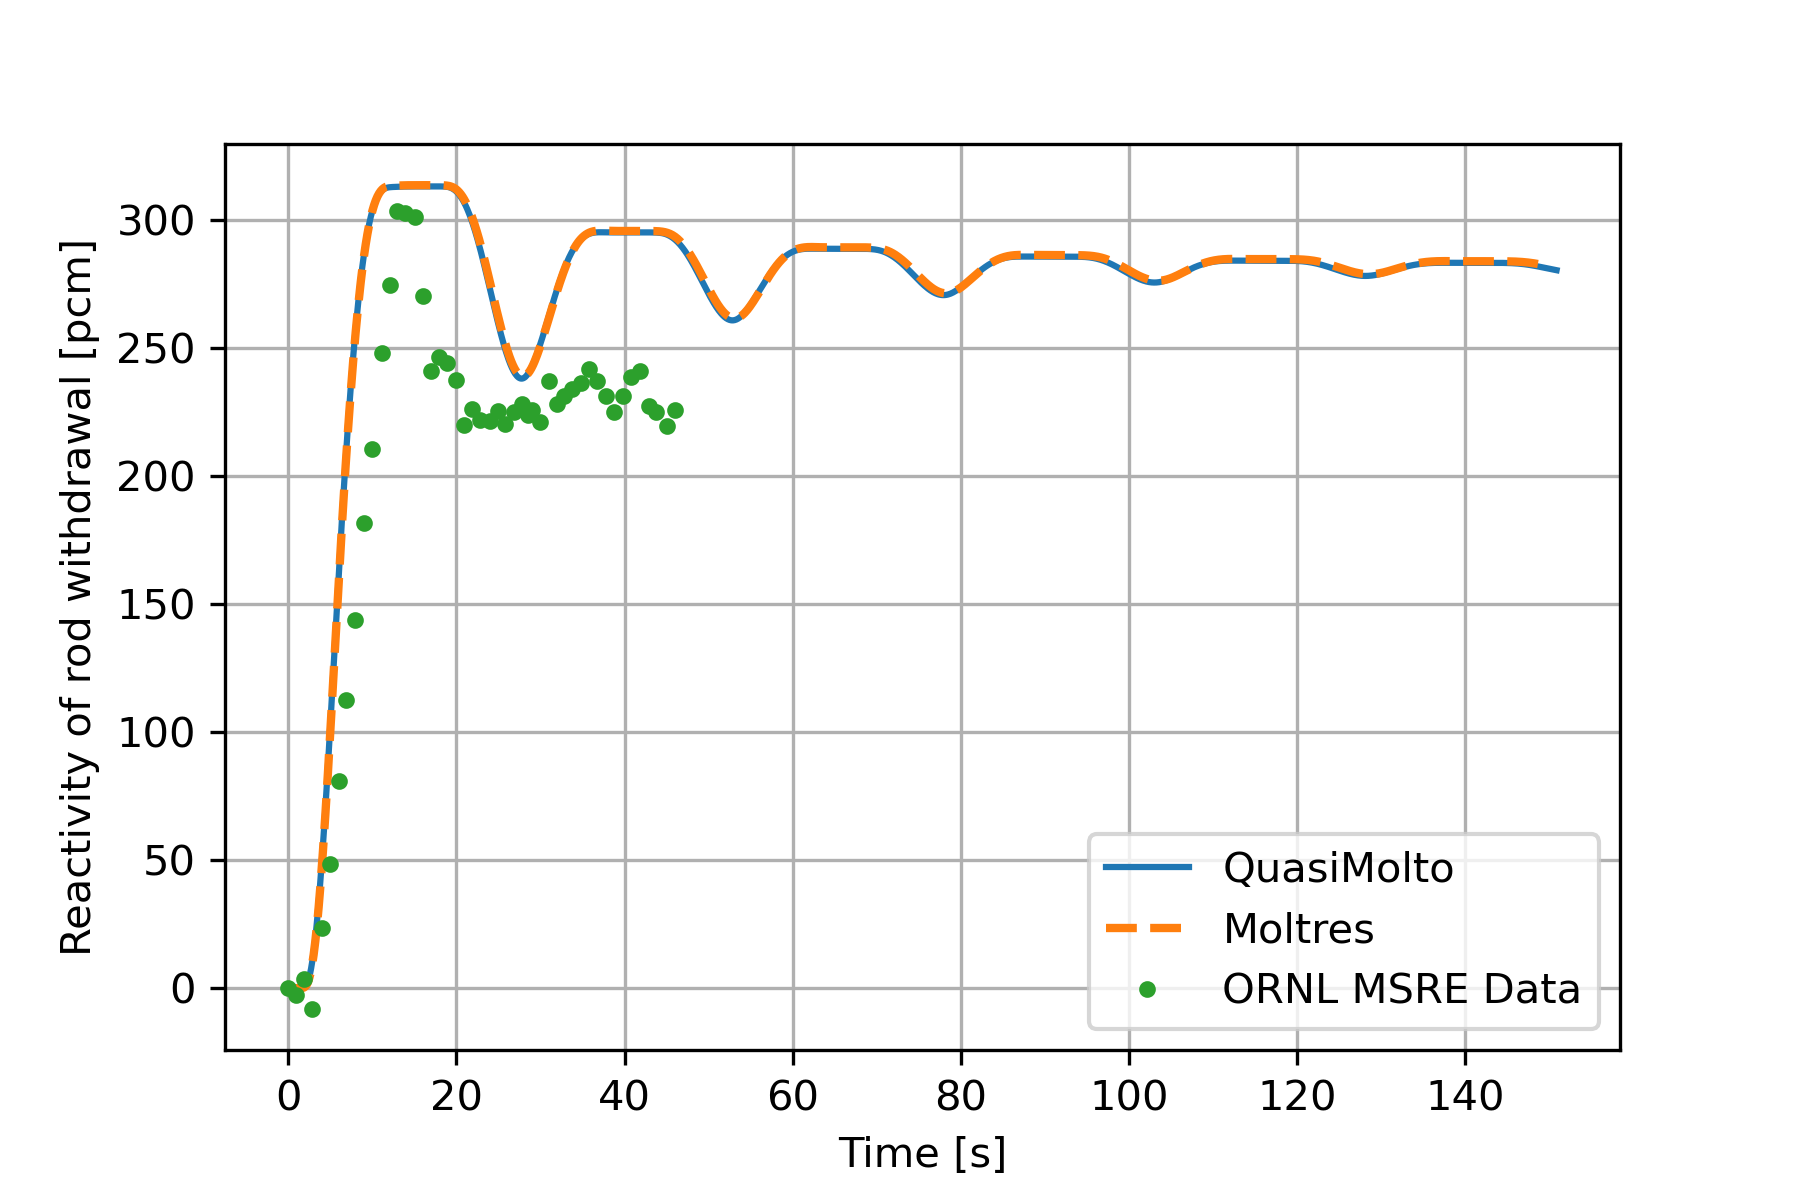
\includegraphics[width=.9\columnwidth]{images/start-up-v2-reactivity}
      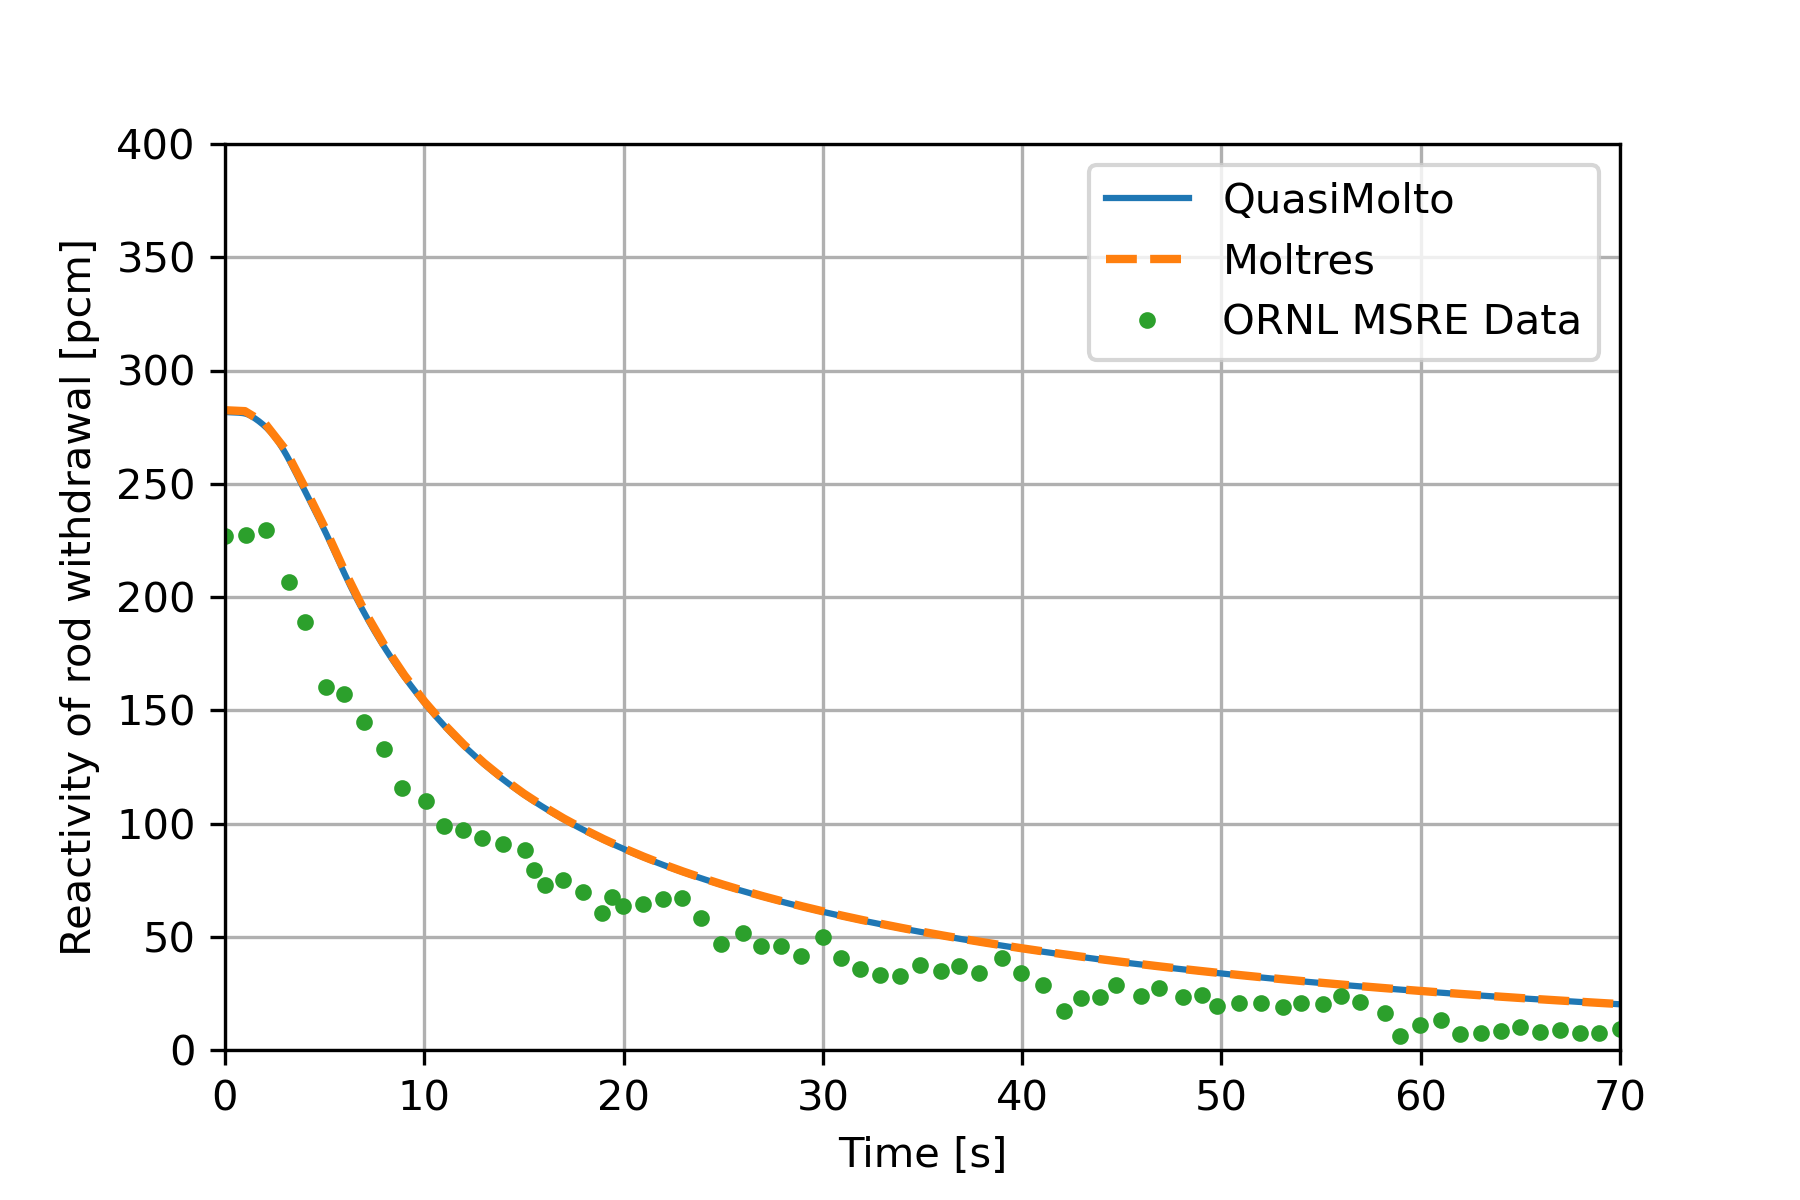
\includegraphics[width=.9\columnwidth]{images/coast-down-v2-reactivity}
      \caption{Reactivity change during the pump start-up (top) and coast-down (bottom)
      transients.}
    \end{figure}
  \end{columns}
\end{frame}

